\documentclass[a4paper,12pt]{report}
\usepackage{multicol}
\usepackage{graphicx}
% Title Page

\makeatletter
\newcommand\ackname{Acknowledgements}
\if@titlepage
  \newenvironment{acknowledgements}{%
      \titlepage
      \null\vfil
      \@beginparpenalty\@lowpenalty
      \begin{center}%
        \bfseries \ackname
        \@endparpenalty\@M
      \end{center}}%
     {\par\vfil\null\endtitlepage}
\else
  \newenvironment{acknowledgements}{%
      \if@twocolumn
        \section*{\abstractname}%
      \else
        \small
        \begin{center}%
          {\bfseries \ackname\vspace{-.5em}\vspace{\z@}}%
        \end{center}%
        \quotation
      \fi}
      {\if@twocolumn\else\endquotation\fi}
\fi
\makeatother

\newcommand{\HRule}{\rule{\linewidth}{0.5mm}}

\begin{document}

\begin{titlepage}

\begin{center}

% Upper part of the page

\includegraphics[width=0.33\textwidth]{./logo}\\[1cm]    

\textsc{\LARGE Indian Institute of Technolgy, Kanpur}\\[1.5cm]

\textsc{\Large ENG 451 Global Communication}\\[0.5cm]

% Title
\HRule \\[0.4cm]
{ \huge \bfseries Effective Communication at Job Interviews}\\[0.4cm]
\HRule \\[1.5cm]

% Author and supervisor
\begin{minipage}{0.4\textwidth}
\begin{flushleft} \large
\emph{Author:}\\
Anirudh \textsc{Kumar}\\
\normalsize
Serial number 24\\
Y9088
\end{flushleft}
\end{minipage}
\begin{minipage}{0.4\textwidth}
\begin{flushright} \large
\emph{Supervisor:} \\
Dr.~T \textsc{Ravichandran}\\
\normalsize
Associate Professor,\\
IIT Kanpur
\end{flushright}
\end{minipage}

\vfill

% Bottom of the page
{\large \today}

\end{center}

\end{titlepage}


\begin{abstract}
Job Interview is an inevitable criterion for selection of a good candidate for a job position. This paper aims at introducing various aspects
of the most common types of Job Interviews and a few points to keep in mind while sitting for a job interview.
\paragraph{}
It first throws light upon the importance and need to prepare for the interview beforehand. Then it mentions the
things to do before and interview. It then proceeds to discuss the various skills and manners required during the interview itself 
and finally mentions a few tips for ensuring the success of interview in the post interview phase.
\paragraph{}
Two appendices are also included which deal with the topics `Technical Knowledge vs. Communication Skills'
and `Interviewer Biases'.
\end{abstract}

\begin{acknowledgements}
I take the privilege of thanking the instructor of the course ENG451, Dr. T. Ravichandran
for introducing me as well as other classmates to the Effective Communication Skills
 in day to day life. His guidance and advice has been a lot of help in preparing this project report.
\paragraph{}
I would also like to thank my friends especially Hunaid, who were a part of the placement process in
2011-2012 and other seniors who provided me with their valuable suggestions for
the survey portion of the report. Without them, the survey and analysis could never have
been done.
\end{acknowledgements}

\tableofcontents
\addcontentsline{toc}{chapter}{Abstract}
\addcontentsline{toc}{chapter}{Acknowledgements}
\addcontentsline{toc}{chapter}{Contents}

\chapter{Job Interviews}             % chapter 1
\section{Introduction}             % section 1.1
Job interview is a meeting between an eligible candidate who is looking for a position in an organization and a recruiter who has been 
given the responsibility to select the most appropriate person for the particular job. It is an opportunity for both the aforementioned 
parties to know each other and fulfill the purpose. \\This project report focuses on the candidate side of the Job interview and how should a person
present himself/herself to the interviewer in order to increase his/her chances of getting the job offer.
As the author of a best selling book on job interviews, `Matthew DeLuca` \cite{matthewluca} says--
{\bf It is not necessarily the best candidate who gets the job offer--it is most likely the best interviewee}. It deals with two
main kind of interviews Telephonic and Personal, and discusses the verbal and non verbal aspects of both.\\
I have also included two sections in the appendix which are not directly related to ones success at Job interviews
but are more of informative nature for candidates sitting in an interview.
\section{More on Job Interviews}       % section 1.2
\subsection{Process}                   % subsection 1.2.1
The process of hiring a candidate begins with a round for shortlisting eligible candidates based on their CV or
a test conducted by the company. GD's may be scheduled for further refining the candidates, but this practice
varies for different organizations. This is followed by a series of interviews: Technical or HR. Both of these have their own specific
methods of preparation, yet the underlying principles for effective communication at both of these interviews is the same.\\
A typical job interview can last for anything around 10 minutes to as long as a few hours. It can be conducted face to face,
 i.e. a personal interview or over a telecommunication medium like a phone or over a video conference on software such as Skype.\\
A bulk of the time in spent by the recruiter in assessing the candidate by asking questions about his work history, style of work, personality,
and any other quality relevant to the position itself. A job interview is a dynamic process for both the parties involved.
An interviewee may predict to an extent whether the interview is going successfully or not and on the other hand the interviewer
may learn something new about the interviewee which was not mentioned by him prior to the interview. So,
due to the dynamic nature of interviews the thoughts and behavior of both sides constantly changes and
this subsequently affects their later thoughts and behavior.\\End of the interview may feature the recruiter encouraging the candidate to pose
any questions to him. Such questions are highly encouraged as they depict an individuals interest in the company and work position offered to him.\\
The process finishes after all the eligible candidates have been interviewed and the recruiting team has assessed them.
Although the assessing may depend on some of the previous achievements or the tests given by the candidate prior to the interview, but the interview
is still remains the major contributor to the selection of a particular individual for a position.


\chapter{Classification of a Job interview}           % chapter 2
\section{Telephonic}     % section 2.1
\subsection{Introduction}  % subsection 2.1.1
Telephonic interviews, as is clear by the name, take place over a communication medium such as telephone.
They are increasingly becoming popular in today's times as the number of applicants is growing.
\subsubsection{Advantages}
With a very large number of applicants, usually a recruiter may want to reduce the number of applicants by interviewing all of them over telephone and eliminating
some of them beforehand. Telephonic interviews are cheaper to conduct than a traditional personal interview and far more convenient
for both parties than their counterparts and are preferred by smaller companies and start-ups. They are also very useful when the interviewer is unable to be physically
present to conduct the interview, eg. him being in other state or country.
\subsubsection{Disadvantages}
But a telephonic interview has some obvious disadvantages also. If the interview is technical there is no
means to put a check on cheating by the candidate unless a video conferencing takes place. Communication problems
may hamper the conduction of a telephonic interview. In a telephonic interview, the interviewer is unable to
judge all the qualities and shortcomings of the candidate as the non-verbal part is mostly absent.
\subsubsection{}
Despite of these shortcomings, the advantages of telephonic interviews generally advocate the need to focus
on them and prepare for them.
\section{Personal}         % section 2.2
\subsection{Introduction}  % subsection 2.2.1
This is the most common and effective type of interview in terms of selecting the best individual for the job.
The candidate faces a single or a panel of interviewers face to face. 
\subsubsection{Advantages}
The interviewers analyze every non-verbal
and verbal gesture of the candidate to decide amongst the best. This allows gathering far more information
about each other for both parties and helps them to perform better. The recruiter can elicit more in-depth response
or help the candidate by filling in information. The question of cheating is also gone as the recruiter observes every move
of the candidate.
\subsubsection{Disadvantages}
Yet it has certain disadvantages too. Most people are afraid of face to face interviews and may not perform well
during the interview, even if they are best suited for the job. It also costs the organization a lot of time and
money to conduct a personal interview which is not desirable for the newer companies and small start-ups.
\subsubsection{}
Personal interview is a highly formal meeting which expects adequate amount of  maturity from both sides.
Proper dress code should be observed and the interview should take place in a quiet and isolated environment.
Following common etiquettes shows the sincerity level of the candidate. After all it is a question of how much 
is a candidate able to demonstrate to the recruiter his suitability for the job.
\subsection{Classification}
A personal interview may be further divided into these following categories based on kinds of questions asked:
\subsubsection{Technical Interview}
Sitting in the interview for a technical position obviously requires certain level of technical knowledge. The level
varies from company to company. Some interviewers may require you to solve hard and mind teasing puzzles, some may ask 
for solving a particular problem, while some may ask you to explain your technical projects to them. The bottom-line is
that you need to prepare extensively for interviews of such companies. \\But your communication skills still
play a vital role here. e.g. you may know the answer to a problem but if you have trouble explaining it to the
recruiter, that counts as a negative for you. 
\subsubsection{HR Interview}
HR interview are designed specifically for testing the soft skills of the candidates. They may also feature questions
which ask for the applicant's managerial skills and behavioral skills. The interviewer may pose a business problem 
and ask a solution for it. This specifically comes under case study questions. These kind of questions are meant to
analyze the creativity, analytical thinking and general knowledge of the candidate.\\
These interviews are conducted by the Human Resource department of the company, hence the name. They are non-technical 
in nature and some of the typical questions asked are:
\begin{itemize}
 \item Tell me about yourself.
 \item Where do you see yourself in 5/10 years from now?
 \item What are your strengths and weaknesses?
\end{itemize}

\chapter{Telephonic Interviews}
\section{Pre-Interview Phase}
As mentioned in earlier chapter telephonic interview is mostly a screening phase before the final interview. But still some
smaller companies and start-ups or any out-station interviewee may it as sole criteria for offering job position. Following points should
be taken care of before the telephonic interview starts.
\subsubsection{Collect information about the company}
Candidates should collect as much information as they can about the company before the interview. It has
a very positive impact at the time of the interview if the candidate is able to discuss the recent events at
the company during the post-interview phase. Various media sources and the company website can be used to
collect such information.
\subsubsection{Prepare common questions}
Most of the telephonic interviews begin with a small introduction of the candidate, so it is wise to write
down the answers to such common question. Practicing giving these answers in front of a mirror will certainly
help reduce the anxiety and nervousness at the time of the interview.
\subsubsection{Ensure that your phone is available}
Ensure that your phone is reachable and charged enough to be able to function throughout the interview. A dropped
connection due to the phone being discharged within 10 minutes of the interview will put a bad impression.
\subsubsection{Ensure a quiet environment}
Interviews should always be conducted in a quiet and isolated environment to avoid distractions and noise.
Since most of the telephonic interviews would take place at the room of candidate, he/she should ensure that the environment 
around him at the time of the interview is silent and with minimal noise. Giving an important interview on a 
street with much noise is certainly not going to have good impression on the interviewer.

\section{Interview Phase}
\subsection{Verbal Skills}
\subsubsection{Let the interviewer lead the interview}
Let the interviewer start the interview. It is better to let the interviewer lead the interview. Only answer 
the questions that the interviewer asks, don't over-clarify things unless the interviewer misinterprets any
answer. And never interrupt the interviewer while he/she is speaking, it outs a very negative impact and shows 
you as rude and arrogant.
\subsubsection{Use correct and clear language}
The language that you use at an interview is very important.
Don't use any words that you don't normally use in your vocabulary. At the time of the interview some people
tend to use complicated words just to impress the recruiter. But wrong words at wrong places do more harm than
 the good that the correctly used words do. Also practice on your grammar before interviews, it is another
plus point in the interviews. Final point on the language- be clear in what you say, it may be hard to listen
if you speak softly over the telephone, leading to miscommunication.
\subsubsection{Don't get nervous or feel shy}
Many people get nervous during the interview and feel intimidated if they are interviewing for a post in
a big organization. Then they start making mistakes that they themselves regret later. This is not a good 
thing and interviewee should practice on overcoming these fears before the interview. You can ask for clarifications
on some doubts you have, and this generally encouraged. Asking for a doubt is clearly better than misinterpreting
a question and making a mistake.
\subsubsection{Be concise}
As the time for a telephonic interview is limited, your answers to the questions should be as concise as possible.
But it does not mean that clarity of the answer can be sacrificed for the sake of conciseness. Best way is to
set a time limit in your mind on the length of the answer you are going to give, depending on the total time of the interview.
Try to finish each of your answers in this predicted time limit. eg. for an interview of 15 minutes, try to finish
every answer in at most 5 minutes, leaving time for other questions to be asked.
\subsubsection{Avoid long pauses}
Don't let a pause continue for too long, keep talking something if you are thinking an answer to a technical
question. Explaining your thought process might give the interviewer something to evaluate you. Avoiding pauses
is also important in a telephonic conversation, as they can get awkward for both parties.

\subsection{Non-Verbal Skills}
\subsubsection{Do not take help}
As the interviewer is unable to see the interviewee, temptation to cheat in the interview can take over easily.
But one should refrain from any kind of cheating during the interview. Remember telephonic interviews are generally
only a screening phase, if you are unable to answer the questions now, the questions in next round are probably 
going to be tougher. Moreover, if the interviewer suspects cheating he may blacklist the candidate from ever sitting
again in the interview for the company.
\subsubsection{Maintain correct posture}
Even when the interviewer is unable to see you, you should maintain correct posture and sit upright during a
telephonic interview. It helps in creating a mental image that a serious thing is going on and not just an every
day chat with a friend.
\subsubsection{Don't lie}
Do not about your achievements, abilities, projects in an interview. If the interviewer suspects a lie, he/she
will probe into it unless you accept that you are not knowledgeable as you claimed you were about the topic.
This will count as very bad impression on the interviewer and he/she may simply reject you.
\subsubsection{Be an active listener}
Note down the names of the interviewer, and other information especially something that will help you in 
the personal interview round, if there is one. Addressing the interviewer by his/her name has a positive effect.
Even try to remembers the voices of the interviewer in case a second round takes place.
\section{Post-Interview Phase}
Post interview phase refers to the time after the formal interview is over and the interviewer engages you 
for discussion. This is particularly important phase as you can get some good information from the recruiter
and display your social skills. A few points to observe in this phase are:
\subsubsection{Thank the interviewer}
Remember to thank the interviewer for his/her time at the end of the interview. Also mention that you are interested 
in the opportunity and ask about the next step in the selection process.
\subsubsection{Ask questions}
Ask questions about the organization, the work you are expected to do, the current and most significant work 
going on the organization. Asking questions depicts your interest in the organization and is very much appreciated.
But avoid questions like `What are my chances of getting selected?' or `Did I perform well?'. These questions
show that you are unsure about yourself and lack self-confidence.
\subsubsection{Try to make light conversation}
Making lighter conversation, maybe crack an appropriate joke will always go in your favor. It says about you
that you are confident and not nervous.
\chapter{Personal Interviews}
\section{Pre-Interview Phase}
\section{Interview Phase}
\subsection{Verbal Skills}
\subsection{Non-Verbal Skills}
\section{Post-Interview Phase}
\chapter{Survey}
To get a the statistics and general level of awareness of students of students at IIT Kanpur campus, a
survey was conducted which is publicly available and accessible to all the fourth and fifth year 
students of IIT Kanpur.
\section{Questions}
\begin{enumerate}
 \item Which year are you in?
  \begin{itemize}
   \item Final
   \item Pre-Final
  \end{itemize}
 \item What is your Department?
 \item What is your CPI?
 \item Did you sit for the placement season 2011-2012?
  \begin{itemize}
   \item Yes
   \item No
  \end{itemize}
 \item If yes, did you accept a Job Offer?
  \begin{itemize}
   \item Yes
   \item No
  \end{itemize}
 \item Did you take a core job or a non core Job?
  \begin{itemize}
   \item Yes
   \item No
  \end{itemize}
 \item On a scale of 1 to 5 how much would you say your placement preparation was?
  \begin{multicols}{5}
  \begin{itemize}
   \item 1
   \item 2
   \item 3
   \item 4
   \item 5
  \end{itemize}
  \end{multicols}
 \item On a scale of 1 to 5, indicate your satisfaction with the job offer you got?
  \begin{multicols}{5}
  \begin{itemize}
   \item 1
   \item 2
   \item 3
   \item 4
   \item 5
  \end{itemize}
  \end{multicols}
\end{enumerate}
\section{Results}
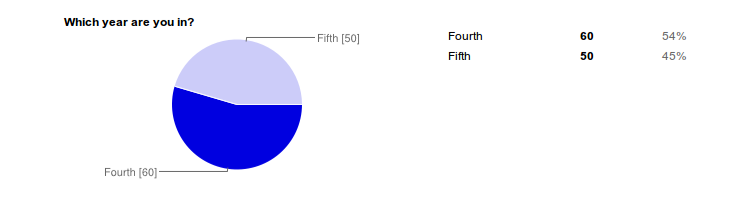
\includegraphics[scale=.5]{1}\\
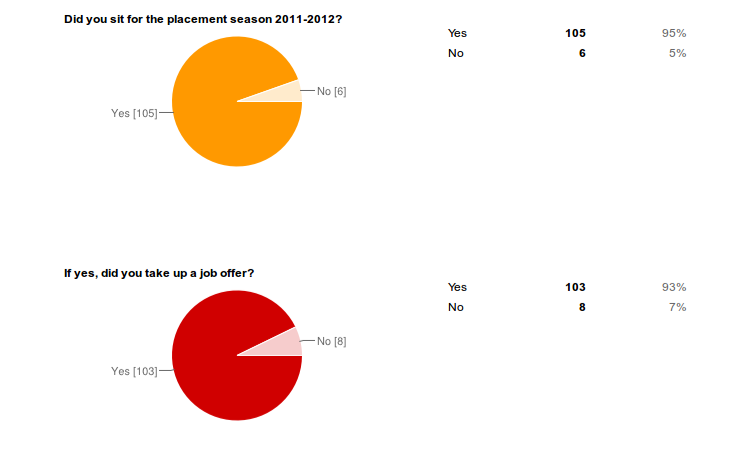
\includegraphics[scale=.5]{2}\\
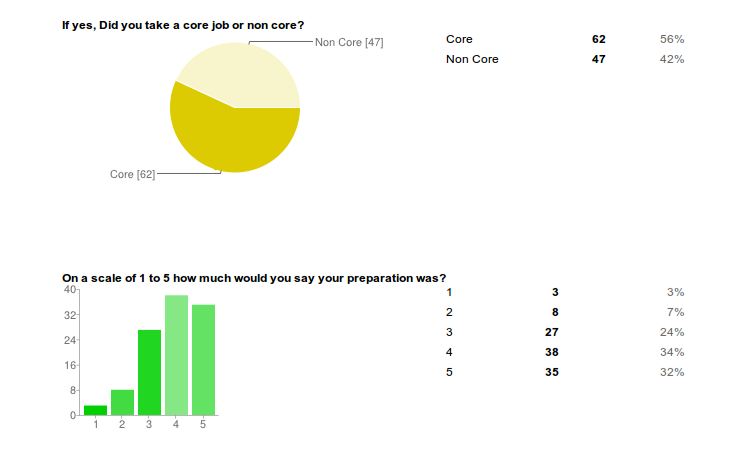
\includegraphics[scale=.5]{3}\\
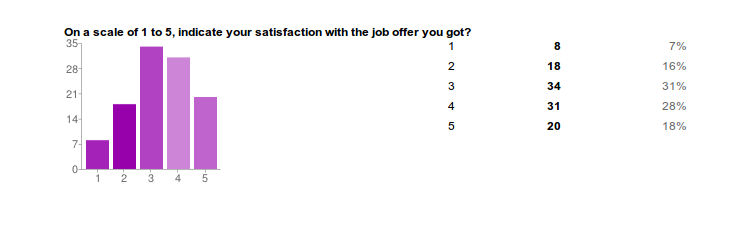
\includegraphics[scale=.5]{4}\\
The average CPI of the people who filled this survey was 7.65
\section{Conclusion}

\appendix
\chapter{Technical Knowledge vs. Communication Skills}
This section is not directly required for Effective Communication but consists of general information on
these topic. Therefore it is included in the appendix as optional reading.
\subsubsection{}
People are not sure whether to concentrate on studies to improve Technical Knowledge or on extra-curricular activities
 to improve Communication Skills. Lets start with a classification for companies into the following two basic sectors:
\begin{itemize}
 \item Core companies
 \item Non-Core companies
\end{itemize}
Core sector includes companies which have a job profile which requires the knowledge one has studied 
while completing his/her education. On the other hand, Non-Core can be defined as all the companies which 
have a job profile which is not related to the education of the candidate. But getting selected for a job
certainly requires some basic knowledge about the work a company does, be it core or non-core.
\subsubsection{}
Now why this classification is important? The main reason is that the preparation for both these sectors
 differs by a fair amount. The Core companies require technical knowledge and may even ignore obvious flaws in
a candidate's communication skills if the technical knowledge is high. The Non-Core companies like consultancies
want their employees to deal with clients and it is absolutely necessary for them to hire candidates with good
soft-skills. Other reason that can be given is that a company can specify whether it belongs to core or non-core
and get suitable candidates for themselves at shortlisting stage to select from.
\subsubsection{}
So the general advise that can be given in this situation is that before while preparing for the placement session 
at campus or applying for jobs off-campus, one should decide beforehand which is the job profile in which he/she would like to work. 
Then go through the job profile of each company and anticipate the qualities required for the job and prepare judiciously.
Since the amount of preparation required is enormous, it is not possible to prepare for both profiles in a short time.

\chapter{Interviewer Biases}
This section throws some light on the shortcomings of the interviewer himself/herself. It talks mainly on the
biased nature of some of the interviewers against or for some candidates. These factors are unrelated to the fact that 
the individual is able to do the job or not, thus their influence should be reduced. This kind of nature is mostly observed in
smaller organizations, but is dependent on the nature of the recruiter and may happen in larger organizations too.
The source of each data is cited in each case.
\paragraph{Gender}
Female candidates tend to score higher scores in interview rounds than their male counterparts with same
level of qualifications if the interviewer is a male\cite{bias}. However, same gender has no effect on these ratings.
\paragraph{Attractiveness}
Physical attractiveness of the applicant is sometimes able to influence the interviewer evaluation scores.
Also if the interviewer has interpersonal attraction\cite{interpersonal} to the interviewee i.e. some interests and ideologies match,
then it is found have an affect on his/her ratings in a positive way.
\paragraph{Cultural differences}
Cultural differences are also found to affect the selection chances of a candidate\cite{bias}. Applicant from 
an ethnic name, accent were viewed less positively by the interviewers than applicants without these traits.
\paragraph{Health}
Unhealthy applicants, particularly those who are highly underweight or severely obese (except, of-course due to some medical condition)
may face discrimination from the hiring team. The reason that can be given is that health is an aspect of an individual
 which can be directly controlled by him/her. As such, the above individuals are seen by the recruiters as lazy, undisciplined and
not motivated and thus non-ideal as a future employee of the organization.
\paragraph{}
Although certain biases like gender, culture and race are prevented by the law, but there can not be a check to the biases
arising from personal attraction and company policies.
The lesson to take from this is that these biases are prevalent and there is no way to stop this from happening,
albeit you can take advantage of these for yourself in certain situations.
\begin{thebibliography}{9}
  \bibitem{matthewluca}
  Matthew DeLuca,
  \emph{Best Answers to the 201 Most Frequently Asked Interview Questions}
  \bibitem{interpersonal}
  Wade and Kinicki (1997),
  \emph{Subjective applicant qualifications and interpersonal attraction as mediators within a process model of interview selection decisions}
  \bibitem{race}
  McFarland, Ryan, Sacco and Kriska (2004),
  \emph{Examination of structured interview ratings across time: The effects of applicant race, rater race, and panel composition}
  \bibitem{bias}
  Purkiss, Perrewé, Gillespie, Mayes and Ferris (2006),
  \emph{Implicit sources of bias in employment interview judgments and decisions}
\end{thebibliography}

\end{document}